% =====================================================================
%  Fig. 3 -- PGSG architecture
%
% ⚠️ 备选实现，**当前未使用**：本地无 LaTeX 环境，Fig. 3 实际由 `_paper_fig3_arch.py`
%    （matplotlib）产出，与其余六张图同规格。本文件留档，将来若要更高排版质量可启用。
%
%  独立编译（推荐，产出裁好边的 PDF，再 \includegraphics 进正文）：
%      pdflatex fig3_architecture.tex
%  产出 fig3_architecture.pdf。
%
%  设计要点（与正文 §4.1 的"证据-决策解耦"一致）：
%    - 上排 = 主特征通路（深蓝）；下排 = 证据通路（砖红）。
%    - 证据只有两条出边，分别进入【尺度轴 transformer 的证据 token】与【门控输入】，
%      绝不并入主通路——这是全图要传达的第一件事。
%    - 零初始化点用 ⓪ 标出，只有【两处】：尺度轴 transformer 的输出投影、门控的末层卷积。
%      证据通路本身**不做**零初始化（它不是残差，梯度经门控零权重回传即可）。
% =====================================================================
\documentclass[tikz,border=4pt]{standalone}
\usepackage{amsmath}
\usetikzlibrary{arrows.meta,positioning,fit,backgrounds,calc}

\definecolor{mainblue}{HTML}{1F4E79}
\definecolor{mainfill}{HTML}{DCE9F5}
\definecolor{evired}{HTML}{A03020}
\definecolor{evifill}{HTML}{F7E3DE}
\definecolor{decipurple}{HTML}{5C3C92}
\definecolor{decifill}{HTML}{E8E1F3}

\begin{document}
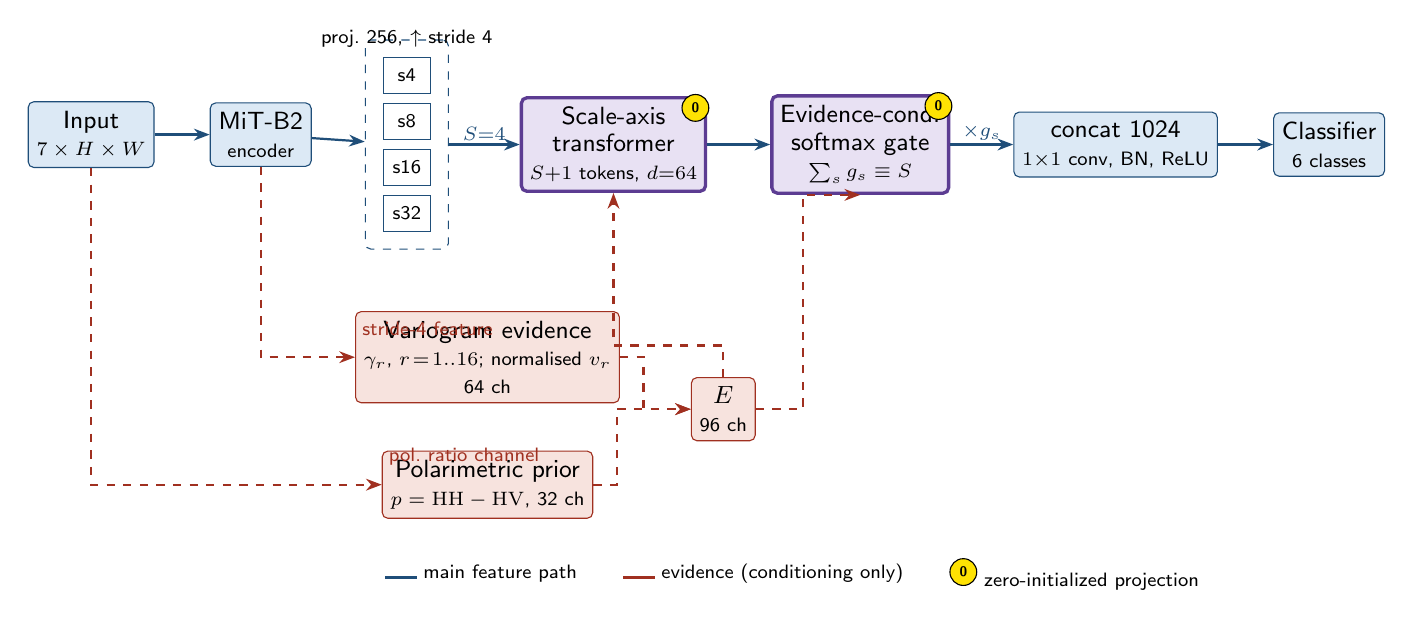
\begin{tikzpicture}[
  font=\sffamily\small,
  >={Stealth[length=2mm]},
  block/.style={draw=mainblue, fill=mainfill, rounded corners=2pt,
                minimum height=8mm, inner xsep=3pt, align=center},
  deci/.style={draw=decipurple, fill=decifill, rounded corners=2pt, very thick,
               minimum height=10mm, inner xsep=3pt, align=center},
  evi/.style={draw=evired, fill=evifill, rounded corners=2pt,
              minimum height=8mm, inner xsep=3pt, align=center},
  feat/.style={draw=mainblue, fill=white, minimum width=6mm,
               minimum height=4.5mm, inner sep=1pt, font=\sffamily\scriptsize},
  mainflow/.style={->, mainblue, thick},
  eviflow/.style={->, evired, thick, dashed},
  lbl/.style={font=\sffamily\scriptsize, inner sep=1pt},
  zero/.style={circle, draw=black, fill=yellow!85!orange, inner sep=0pt,
               minimum size=3.4mm, font=\sffamily\bfseries\tiny}
]

% ---------------------------------------------------------------- 主通路
\node[block] (in) {Input\\[-1pt]\scriptsize $7\times H\times W$};
\node[block, right=7mm of in] (enc) {MiT-B2\\[-1pt]\scriptsize encoder};

% 四个尺度特征
\node[feat, right=9mm of enc, yshift=7.5mm]  (f1) {s4};
\node[feat, below=1.2mm of f1]               (f2) {s8};
\node[feat, below=1.2mm of f2]               (f3) {s16};
\node[feat, below=1.2mm of f3]               (f4) {s32};
\node[lbl, above=0.8mm of f1] {proj.\ 256, $\uparrow$ stride 4};
\begin{scope}[on background layer]
  \node[draw=mainblue, dashed, rounded corners=2pt, inner sep=2.2mm,
        fit=(f1)(f4)] (fbox) {};
\end{scope}

\node[deci, right=9mm of fbox] (xat)
  {Scale-axis\\[-1pt]transformer\\[-1pt]\scriptsize $S{+}1$ tokens, $d{=}64$};
\node[deci, right=8mm of xat] (gate)
  {Evidence-cond.\\[-1pt]softmax gate\\[-1pt]\scriptsize $\sum_s g_s\equiv S$};
\node[block, right=8mm of gate] (fuse)
  {concat 1024\\[-1pt]\scriptsize $1{\times}1$ conv, BN, ReLU};
\node[block, right=7mm of fuse] (cls) {Classifier\\[-1pt]\scriptsize 6 classes};

\draw[mainflow] (in)  -- (enc);
\draw[mainflow] (enc) -- (fbox);
\draw[mainflow] (fbox) -- node[lbl, above] {$S{=}4$} (xat);
\draw[mainflow] (xat) -- (gate);
\draw[mainflow] (gate) -- node[lbl, above] {$\times g_s$} (fuse);
\draw[mainflow] (fuse) -- (cls);

% ---------------------------------------------------------------- 证据通路
\node[evi, below=15mm of xat, xshift=-16mm] (vario)
  {Variogram evidence\\[-1pt]\scriptsize $\gamma_r$, $r\!=\!1..16$; normalised $v_r$\\[-1pt]\scriptsize 64 ch};
\node[evi, below=6mm of vario] (pol)
  {Polarimetric prior\\[-1pt]\scriptsize $p=\mathrm{HH}-\mathrm{HV}$, 32 ch};
\node[evi, right=9mm of vario, yshift=-6.6mm] (E)
  {$E$\\[-1pt]\scriptsize 96 ch};

\draw[eviflow] (vario.east) -- ++(3mm,0) |- (E.west);
\draw[eviflow] (pol.east)   -- ++(3mm,0) |- (E.west);

% 证据来源：encoder stride-4 特征 / 输入的极化比通道
\draw[eviflow] (enc.south) |- (vario.west);
\draw[eviflow] (in.south)  |- (pol.west);
\node[lbl, evired, right=0.5mm of vario.west, yshift=3.6mm] {stride-4 feature};
\node[lbl, evired, right=0.5mm of pol.west, yshift=3.6mm] {pol.\ ratio channel};

% 证据 -> 两个决策模块（唯一的两条出边）
\draw[eviflow] (E.north) -- ++(0,4mm) -| (xat.south);
\draw[eviflow] (E.east)  -- ++(6mm,0) |- (gate.south);

% ---------------------------------------------------------------- 零初始化标记
\node[zero] at ($(xat.north east)+(-1.5mm,-1.5mm)$)  {0};
\node[zero] at ($(gate.north east)+(-1.5mm,-1.5mm)$) {0};

% ---------------------------------------------------------------- 图例
\node[lbl, anchor=west] (lg1) at ($(pol.south west)+(0,-7mm)$)
  {\textcolor{mainblue}{\rule{4mm}{1pt}}\ main feature path};
\node[lbl, anchor=west, right=5mm of lg1] (lg2)
  {\textcolor{evired}{\rule{4mm}{1pt}}\ evidence (conditioning only)};
\node[lbl, anchor=west, right=5mm of lg2] (lg3)
  {\tikz\node[zero]{0};\ zero-initialized projection};

\end{tikzpicture}
\end{document}
